%\documentclass{article}
%
%\usepackage{fancyhdr}
%\usepackage{extramarks}
%\usepackage{amsmath}
%\usepackage{amsthm}
%\usepackage{amsfonts}
%\usepackage{tikz}
%\usepackage{enumerate}
%\usepackage{graphicx}
%\graphicspath{ {images/} }
%\usepackage[plain]{algorithm}
%\usepackage{algpseudocode}
%\usepackage[document]{ragged2e}
%\usepackage{textcomp}
%\usepackage{color}   %May be necessary if you want to color links
%\usepackage{import}
%\usepackage{hyperref}
%\hypersetup{
%    colorlinks=true, %set true if you want colored links
%    linktoc=all,     %set to all if you want both sections and subsections linked
%    linkcolor=black,  %choose some color if you want links to stand out
%}
%
%\usetikzlibrary{automata,positioning}
%
%
%% Basic Document Settings
%
%
%\topmargin=-0.45in
%\evensidemargin=0in
%\oddsidemargin=0in
%\textwidth=6.5in
%\textheight=9.0in
%\headsep=0.25in
%\setlength{\parskip}{1em}
%
%\linespread{1.1}
%
%\pagestyle{fancy}
%\lhead{\hmwkAuthorName}
%\lfoot{\lastxmark}
%\cfoot{\thepage}
%
%\renewcommand\headrulewidth{0.4pt}
%\renewcommand\footrulewidth{0.4pt}
%
%\setlength\parindent{0pt}
%
%
%\newcommand{\hmwkTitle}{Math Review Notes---Real Analysis}
%\newcommand{\hmwkAuthorName}{\textbf{G. Faletto} }
%
%
%%%%%% Title Page
%
%
%\title{
%    \vspace{2in}
%    \textmd{\textbf{ \hmwkTitle}}\\
%}
%
%\author{Gregory Faletto}
%\date{}
%
%\renewcommand{\part}[1]{\textbf{\large Part \Alph{partCounter}}\stepcounter{partCounter}\\}
%
%
%%%%%% Various Helper Commands
%
%
%%%%%% Useful for algorithms
%\newcommand{\alg}[1]{\textsc{\bfseries \footnotesize #1}}
%
%%%%%% For derivatives
%\newcommand{\deriv}[2]{\frac{\mathrm{d} #1}{\mathrm{d} #2}}
%
%%%%%% For partial derivatives
%\newcommand{\pderiv}[2]{\frac{\partial #1}{\partial #2}}
%
%%%%%% Integral dx
%\newcommand{\dx}{\mathrm{d}x}
%
%%%%%% Alias for the Solution section header
%\newcommand{\solution}{\textbf{\large Solution}}
%
%%%%%% Probability commands: Expectation, Variance, Covariance, Bias
%\newcommand{\E}{\mathbb{E}}
%\newcommand{\Var}{\mathrm{Var}}
%\newcommand{\Cov}{\mathrm{Cov}}
%\newcommand{\Bias}{\mathrm{Bias}}
%\newcommand\indep{\protect\mathpalette{\protect\independenT}{\perp}}
%\def\independenT#1#2{\mathrel{\rlap{$#1#2$}\mkern2mu{#1#2}}}
%\DeclareMathOperator{\Tr}{Tr}
%
%\theoremstyle{definition}
%\newtheorem{theorem}{Theorem}
%\theoremstyle{definition}
%\newtheorem{proposition}[theorem]{Proposition}
%\theoremstyle{definition}
%\newtheorem{lemma}[theorem]{Lemma}
%\theoremstyle{definition}
%\newtheorem{corollary}{Corollary}[theorem]
%\theoremstyle{definition}
%\newtheorem{definition}{Definition}[section]
%\newtheorem*{remark}{Remark}
%
%%%%%% Tilde
%\newcommand{\textapprox}{\raisebox{0.5ex}{\texttildelow}}
%
%\begin{document}
%
%\maketitle
%
%\pagebreak
%
%\tableofcontents
%
%\
%
%\
%
%\begin{center}
%Last updated \today
%\end{center}
%
%
%
%\newpage
%
%%
%%
%%
%%
%%
%%
%%
%%
%%%
%% Real Analysis

% Real Analysis
\section{Real Analysis}

These are my notes from Math 4650: Analysis I at Cal State LA as well as Prof. Steven Heilman's notes from Math 541A at USC.

%\textbf{Brush up on recent real analysis (especially open, closed, compact, etc)}

%Midterm 1
\subsection{Midterm 1}

% Homework 1
\subsubsection{Homework 1}

\textbf{Definition:} Let \(S \subseteq \mathbb{R}\). We say that \(S\) is \textbf{bounded from above} if \(\exists \ b \in \mathbb{R}\) where \[s \leq b \ \forall \ s \in S\]If this is the case, we call \(b\) an \textbf{upper bound} of \(S\).

If \(b \leq c \) for all upper bounds \(c\) of \(S\), we call \(b\) the \textbf{supremum} of \(S\): \(b = \sup(S)\).

We say that \(S\) is \textbf{bounded from below} if \(\exists \ a \in \mathbb{R}\) where \[s \geq a \ \forall \ s \in S\]If this is the case, we call \(a\) a \textbf{lower bound} of \(S\).

If \(a \geq d \) for all lower bounds \(d\) of \(S\), we call \(a\) the \textbf{infimum} of \(S\): \(a = \inf(S)\).

\textbf{Useful Sup/Inf Fact:} Let \(S \in \mathbb{R}\), \(S \neq \emptyset\). 

\begin{enumerate}[(1)]

\item Suppose \(S\) is bounded from above by an element \(b\). Then \(b = \sup(S) \iff \forall \ \epsilon >0 \ \exists \ x \in S\) with \[b - \epsilon < x \leq b\]

\item Suppose \(S\) is bounded from below by an element \(a\). Then \(a = \inf(S) \iff \forall \ \epsilon >0 \ \exists \ x \in S\) with \[a \leq x < a + \epsilon\]

\end{enumerate}

\textbf{Completeness Axiom}: Let \(S\) be a nonempty subset of \(\mathbb{R}\). If \(S\) is bounded from above, then \(\sup(S)\) exists. If \(S\) is bounded from below, then \(\inf(S)\) exists.

%\[
%|x - y| < \epsilon \iff y - \epsilon < x < y + \epsilon
%\]

\textbf{Facts about absolute value:}

\begin{enumerate}[(1)]

\item \(|x-y| < \epsilon \iff y - \epsilon < x < y + \epsilon\) (proof: in notes 08/23)

\item \(|ab| = |a||b|\) (proof: 7(c) in Homework 1)

\item Let \(\epsilon >0\). Then \(|a| < \epsilon \iff -\epsilon < a < \epsilon\). (Proof: follows from (1) if \(x = a\), \(y = 0\).)

\item \(-|a| \leq a \leq |a|\) (proof: Follows from (1) if \(x = a\), \(y = 0\), \(\epsilon = |a|\).)

\item \textbf{Triangle Inequality:} \(|a + b| \leq |a| + |b|\) (Proof in notes 08/23)

\item \(|\ |a| - |b| \ | \leq |a - b|\) (Proof: 7(d) in Homework 1)

\item \textbf{Triangle Inequality:} \(|a - b| \leq |a| + |b|\) (Proof: follows from (5), let \(b = -b\).)

\item If \(a < x < b\) and \(a < y < b\) then \(|x - y| < b - a\). (Proof: 7(a) in Homework 1)

\item \(|a - b| = |b - a|\) (Proof: 7(b) in Homework 1.)

\end{enumerate}

% Homework 2
\subsubsection{Homework 2}

\textbf{Definition:} A sequence \((a_n)\) of real numbers is said to \textbf{converge} to a \textbf{limit} \(L \in \mathbb{R}\) if \(\forall \ \epsilon > 0 \ \exists \ N > 0 \) where

\[
n \geq N \implies |a_n - L| < \epsilon
\]

We say that \((a_n)\) \textbf{diverges} if it does not converge.

\textbf{Definition:} A sequence \((a_n)\) of real numbers is \textbf{bounded} if \(\exists \ M > 0\) where \(\forall \ n \in \mathbb{N}\) \[\ |a_n| \leq M \]

\textbf{Theorem.} If \((a_n)\) converges then \((a_n)\) is bounded.

\textbf{Definition:} Let \((a_n)\) be a sequence of real numbers. We say that \((a_n)\) is a \textbf{Cauchy sequence} if \(\forall \ \epsilon > 0 \ \exists \ N\) where

\[
n, m \geq N \implies |a_n - a_m| < \epsilon
\]

\textbf{Theorem.} \((a_n)\) is Cauchy if and only if \((a_n)\) converges.

\textbf{Corollary.} If \((a_n)\) is Cauchy then \((a_n)\) is bounded.

\pagebreak

% Midterm 2
\subsection{Midterm 2}

% Homework 3
\subsubsection{Homework 3}

\textbf{Limits of functions at infinity.} Let \(f\) be a real-valued function defined on some set \(D\) where \(D\) contains an interval of the form \((a, \infty)\). Let \(L \in \mathbb{R}\). We say \[\lim_{x \to \infty} f(x) = L\]if \(\forall \ \epsilon >0 \ \exists \ N \in \mathbb{R}\) where

\[
x \geq N \implies |f(x) - L| < \epsilon
\]

\textbf{Definition:} Let \(D \subseteq \mathbb{R}\). Let \(a \in \mathbb{R}\). We say that \(a\) is a \textbf{limit point} (or ``cluster point," or ``accumulation point") of \(D\) if \(\forall \ \delta > 0 \ \exists \ x \in D\) where

\[
x \neq a \text{ and } |x - a| < \delta
\]

(Note that \(a\) may or may not be contained in \(D\).)

\textbf{Limit of a function at \(a\)}: Let \(D \subseteq \mathbb{R}\) and \(f:d \to \mathbb{R}\). Let \(a\) be a limit point of \(D\). Let \(x \in D\). We say that \(f\) has a \textit{limit as \(x\) tends to \(a\)} if \(\exists \ L \in \mathbb{R}\) where \(\forall \ \epsilon > 0 \ \exists \ \delta > 0 \) such that

\[
0 < |x - a| < \delta \implies |f(x) - L| < \epsilon
\]

and we write \[\lim_{x \to a} f(x) = L\]

\textbf{Properties of Limits:} Let \(D \in \mathbb{R}\) and let \(a\) be a limit point of \(D\). Suppose \(f:D \to \mathbb{R}\) and \(g: D \to \mathbb{R}\). Let \(\alpha \in \mathbb{R}\).

\begin{enumerate}[(1)]

\item If \(\lim_{x \to a} f(x) = L\) and \(\lim_{x \to a} g(x) = M\) then

\begin{enumerate}[(a)]

\item \[\lim_{x \to a} \alpha = \alpha\]

\item \[\lim_{x \to a} [f(x) + g(x)] = L + M\]

\item \[\lim_{x \to a} [f(x) - g(x)] = L - M\]

\item \[\lim_{x \to a} [f(x) \cdot g(x)] = L \cdot M\]

\item \[\lim_{x \to a} [\alpha \cdot f(x)] = \alpha \cdot L\]

\end{enumerate}

\item If \(h:D \to \mathbb{R}\) and \(h(x) \neq 0 \ \forall \ x \in D\) and \(\lim_{x \to a} h(x) = H \neq 0\), then

\[
\lim_{x \to a} \frac{1}{h(x)} = \frac{1}{H}
\]

Note that properties (2) and (1)(d) combined imply

\[
\lim_{x \to a} \frac{f(x)}{h(x)} = \frac{L}{H}
\]

\end{enumerate}

% Homework 4
\subsubsection{Homework 4}

\textbf{Continuity:} Let \(D \subseteq \mathbb{R}\) and \(f:D \to \mathbb{R}\) and \(a \in D\). Then \(f\) is \textbf{continuous} at \(a\) if \(\lim_{x \to a} f(x)\) exists and 

\[
\lim_{x \to a} f(x) = f(a)
\]

(Note: if \(f\) is continuous at \(a\), then we can say \(\forall \ \epsilon > 0 \ \exists \ \delta > 0 \) such that

\[
|x - a| < \delta \implies |f(x) - L| < \epsilon
\]

that is, we don't need to say \(0 < |x - a| < \delta\)).

If \(B \subseteq D\), then \(f\) is \textbf{continuous on B} if \(f\) is continuous at every \(b \in B\).

\textbf{Intermediate Value Theorem:} Let \(f\) be continuous on \([a, b]\) and suppose \(f(a) < f(b)\). \(\forall \ d\) such that \[f(a) < d < f(b)\]  \(\exists \ c \in \mathbb{R}\) where \[a < c < b, \ f(c) = d\]

\pagebreak

% Final
\subsection{Final}

% Homework 5
\subsubsection{Homework 5}

\textbf{Definition:} Let \(S \subseteq \mathbb{R}\). We say \(x \in \mathbb{R}\) is an \textbf{interior point} of \(S\) if there exists an open interval \((a, b)\) where \[x \in (a, b) \text{ and } (a, b) \subseteq S\]

\textbf{Open sets:} Let \(S \subseteq \mathbb{R}\). We say \(S\) is \textbf{open} if every \(x \in S\) is an interior point of \(S\).

\textbf{Closed sets:} Let \(S \subseteq \mathbb{R}\). We say \(S\) is \textbf{closed} if \(\mathbb{R} \setminus S\) is open.

\textbf{Theorem.} A set is closed if and only if it contains all of its limit points.

\textbf{Facts about open and closed sets:} Suppose \(a, b \in \mathbb{R}\). Then

\begin{itemize}

\item \((a, \infty)\) is open (Proof: Homework 5 problem 5b).

\item \((-\infty, b)\) is open (Proof: Homework 5 problem 5a).

\item \((a, b)\) is open (Proof: class notes).

\item If \(a < b\), then \([a, b]\) is closed (Proof: Homework 5 problem 5c).

\item If \(A\) and \(B\) are open, then \(A \cup B\) and \(A \cap B\) are open (Proof: Homework 5 problem 3).

\item If \(A\) and \(B\) are closed, then \(A \cup B\) and \(A \cap B\) are closed (Proof: Homework 5 problem 4).

\item \(\mathbb{R}\) is open (Proof: Homework 5 problem 1) and closed (Proof: \(\mathbb{R} \setminus \mathbb{R} = \emptyset\) is open).

\item \(\emptyset\) is open (Proof: Homework 5 problem 2) and closed (Proof: \(\mathbb{R} \setminus \emptyset = \mathbb{R}\) is open).

\end{itemize}

\textbf{Definition:} Let \(S \subseteq \mathbb{R}\). An \textbf{open cover} of \(S\) is a collection \(X = \{\mathcal{O}_\alpha \ | \ \alpha \in I \} \) where each set \(\mathcal{O}_\alpha\) is an open subset of \(\mathbb{R}\) such that

\[
S \subseteq \bigcup_{\alpha \in I} \mathcal{O}_\alpha
\]

(Here \(I\) is some set that indexes the \(\mathcal{O}_\alpha\)).

If \(X' \subseteq X\) such that \[S \subseteq  \bigcup_{\mathcal{O}_\alpha \in X'} \mathcal{O}_\alpha\]then \(X'\) is called a \textbf{subcover} of \(S\) contained in \(X\). In addition, if \(X'\) is finite then we call \(X'\) a \textbf{finite subcover} of \(S\) contained in \(X\).

\textbf{Compactness:} Let \(S \subseteq \mathbb{R}\). We say that \(S\) is \textbf{compact} if every open cover of \(S\) contains a finite subcover. 

\textbf{Definition:} Let \(S \subseteq \mathbb{R}\). We say that \(S\) is \textbf{bounded} if \(\exists \ M > 0\) where \(S \subseteq [-M, M]\).

Note: \(S\) is bounded if and only if \(|s| \leq M\  \forall \ s \in S \).

\textbf{Heine-Borel Theorem.} Let \(S \subseteq \mathbb{R}\). \(S\) is compact if and only if \(S\) is closed and bounded.

%\pagebreak

\textbf{Theorem.} Let \(f: D \to \mathbb{R}\) be continuous on \(D\). If \(X \subseteq D\) and \(X\) is compact (closed and bounded), then

\[
f(\bar{x}) = \{f(x) \ | \ x \in X\}
\]

is compact (closed and bounded).

\textbf{Corollary:} Suppose \(f: D \to \mathbb{R}\) where \(D\) is closed and bounded. Then there exists \(a, b \in D\) where \(f(a)\) is the min of \(f\) on \(D\) and \(f(b)\) is the max of \(f\) on \(D\).

% Homework 6
\subsubsection{Homework 6}

\textbf{Uniform Continuity:} Let \(D \subseteq \mathbb{R}\) and let \(f: D \to \mathbb{R}\). We say that \(f\) is \textbf{uniformly continuous} on \(D\) if \(\forall \ \epsilon > 0 \ \exists \ \delta > 0\) where

\[
x, y \in D \text{ and } 0 < |x - y| < \delta \implies |f(x) - f(y)| < \epsilon
\]

\textbf{Uniform continuity implies continuity.} Suppose \(f:D \to \mathbb{R}\) where \(D \subseteq \mathbb{R}\). If \(f\) is uniformly continuous on \(D\), then \(f\) is continuous at every \(a \in D\).

\subsection{More Theorems}

\begin{theorem}\label{ra.fubini} \textbf{Fubini's Theorem.} Let \(h: \mathbb{R}^2 \to \mathbb{R}\) be a continuous function such that \(\int \int_{\mathbb{R}^2}|h(x,y)| dxdy < \infty\). Then

\[
\int \int_{\mathbb{R}^2} h(x,y)dxdy = \int_{\mathbb{R}} \bigg( \int_{\mathbb{R} } h(x,y)dx \bigg) dy = \int_{\mathbb{R}} \bigg( \int_{\mathbb{R}} h(x,y)dy \bigg) dx
\]

\end{theorem}

\subsection{Problems from Practice Math GRE Subject Tests}

%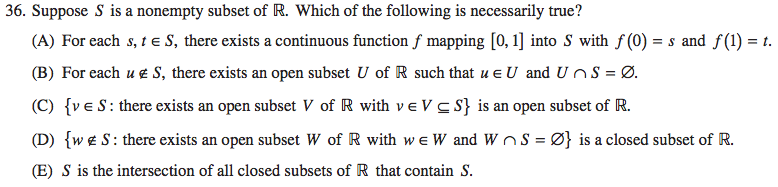
\includegraphics[scale=0.65]{1268_36}
%
%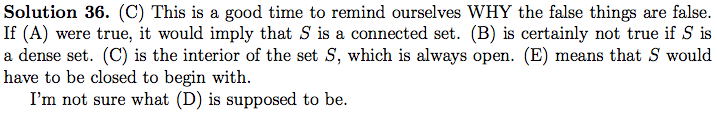
\includegraphics[scale=0.65]{1268_36s}

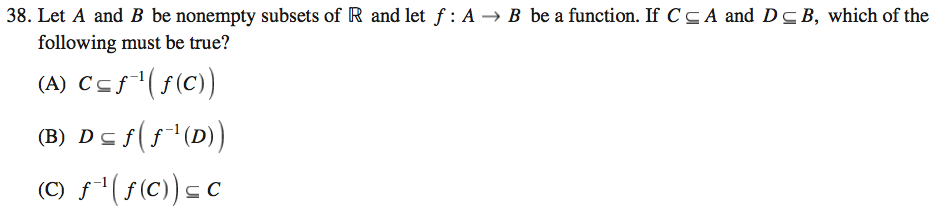
\includegraphics[scale=0.5]{0568_38}

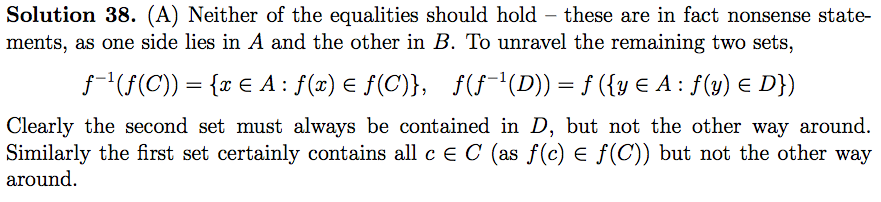
\includegraphics[scale=0.5]{0568_38s}

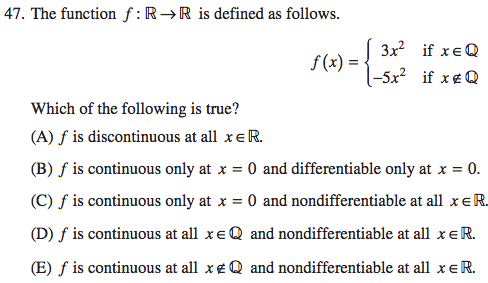
\includegraphics[scale=0.65]{1268_47}

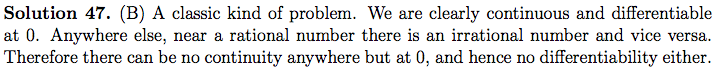
\includegraphics[scale=0.65]{1268_47s}

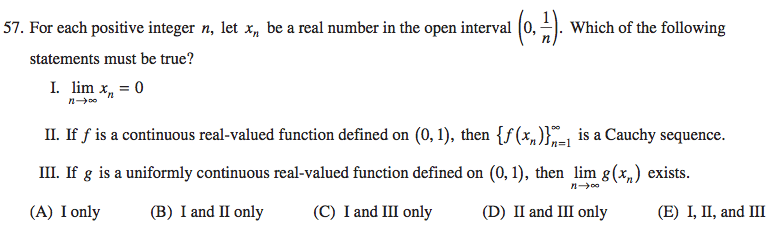
\includegraphics[scale=0.65]{1268_57}

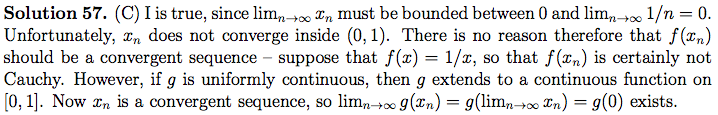
\includegraphics[scale=0.65]{1268_57s}

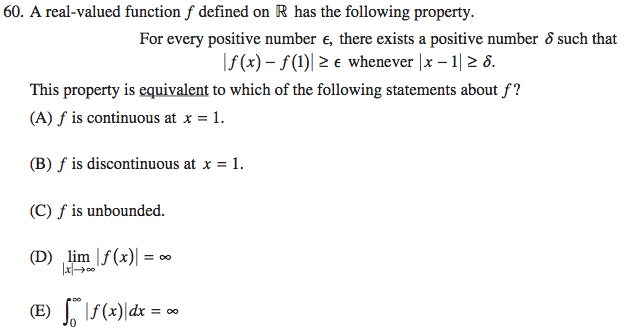
\includegraphics[scale=0.65]{1268_60}

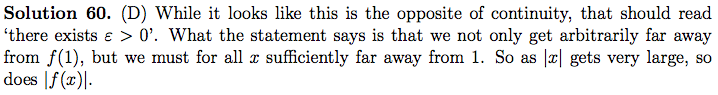
\includegraphics[scale=0.65]{1268_60s}

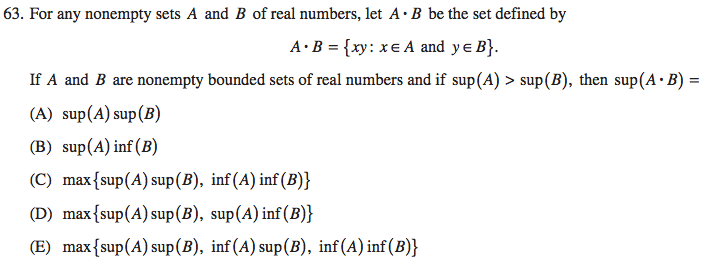
\includegraphics[scale=0.65]{1268_63}

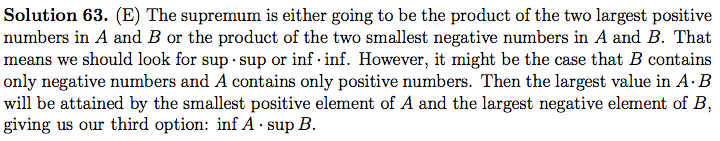
\includegraphics[scale=0.65]{1268_63s}

%\end{document}